\chapter{Lecture 15: Continuous random variables, uniform distribution, and percentiles}
\section{Continuous random variables}
So far, the random variables that we have dealt with have all been discrete; in sections \ref{sec8.10} and \ref{discrete random variable}, we learned that discrete random variables are functions whose outputs specify individual events that can be counted, or listed. The set of outputs of a discrete random variable can always be replaced (i.e., relabelled) by some subset of the natural numbers. \\

\noindent When a random variable corresponds to something that needs to be ``measured'' rather than ``counted,'' it is called \textbf{continuous}. The set of outputs of a continuous random variable can never be mapped to a subset of the natural numbers; instead, they need to be represented by an interval of real numbers. \\

\noindent For example, the number of knots in a fixed length of rope is a discrete random variable; however, the length of a randomly selected piece of rope is a continuous random variable. The number of houses on a randomly selected street is a discrete random variable; but the time that it takes to drive down the street is a continuous random variable.

\subsection{Probability density function} \label{pdf}
The probabilities of a continuous random variable are given by its \textbf{probability density function}, $\boldsymbol{f}$, (often abbreviated \textbf{pdf}). We often use $f$ to represent some arbitrary function; however, in the context of continuous random variables we always use $f$ to represent the pdf \label{f(pdf)}\\

\noindent For $f$ to be a suitable pdf, it must satisfy certain conditions. First of all, it has to be continuous (see section \ref{not have derivatives} about continuity). However, technically it does not have to be continuous over its whole domain; we just need to be able to break its domain up into a union of intervals on which $f$ is continuous. This property is called \textbf{piecewise continuity}. We will not need to concern ourselves too much with piecewise continuity in this course. \\

\noindent Secondly, since $f$ will be used to give probabilities, the way that we use it must also satisfy the 3 probability measure axioms. As usual, axiom 3 is not something we need to check explicitly in this course (we will see, in section \ref{subsec15.1}, that axiom 3 tells us part of how we use the pdf).  Thus we are left with needing to check that
\[
\bullet f(x) \geq 0 \;\; \text{for all} \; x \in \R \tag{equivalent to checking axiom 2}
\]
\[
\bullet \hspace{1cm} \int_{-\infty}^\infty f(t) \; dt = 1 \hspace{0.14cm} \tag{equivalent to checking axiom 1}
\]
When dealing with discrete random variables, we verify axiom 1 by checking that all of the probabilities sum to 1. For a continuous function, the equivalent of this sum is an integral; we want to sum the probabilities associated with all possible outputs, so we integrate from $-\infty$ to $\infty$ when we check axiom 1. We can interpret this condition as requiring that the total area under the graph of a pdf be equal to 1. \\

\noindent Probability density functions are usually specified by a rule, and can be displayed in a graph.

\subsection{Example} \label{ex15.1}
In example \ref{ex13.1} we found the total area under the graph of the following function is equal to 1:
\[
f(x) = \left\{ \begin{array}{ll}
0, & \; \text{if} \; x < 1 \smallskip \\
x - 1, & \; \text{if} \; 1 < x \leq 2 \smallskip \\
3-x, & \; \text{if} \; 2 < x \leq 3 \smallskip \\
0, &  \; \text{if} \; x > 3
\end{array}
\right.
\]
We can also see, from the function rule, that $f(x) \geq 0$ for all $x \in \R$ and that $f$ is continuous. Hence $f$ satisfies all of the conditions to be a probability density function.

\subsection{Using a pdf to give probabilities} \label{subsec15.1}
The values that a discrete random variable takes are always exact. For example, if you are told that success occurred on the $3^\text{rd}$ trial, then there is no mistaking exactly which trial was a success (you know it was exactly the $3^\text{rd}$ trial). \\

\noindent Continuous random variables, on the other hand, are associated with outcomes that can never physically be exact. For example, suppose that you are told that the length of a ruler is 1 meter. Is the ruler \textit{exactly} 1 meter long, or is it perhaps 1.00001 meters long? We could always demand more accuracy from our measurements, and in so doing we eventually must reach the limitations of whichever device that we are using to take the measurements. Even universal constants like the speed of light can only be measured to a limited degree of accuracy. The probability that a continuous random variable takes a single \textit{exact} value, it follows, must always be zero. Hence, rather than ask for $P(X = a)$, for some real number $a$, when $X$ is a continuous random variable, we ask for $P(a < X < b)$; that is, we ask for the probability that $X$ falls within some interval, $(a,b)$, (this interval could be viewed as our desired level of accuracy). \\

\noindent Hence we define
%\noindent In section \ref{pdf} we mentioned that probability measure axiom 3 tells us how to use $f$; this means that we need to come up with a way to interpret the outputs of $f$ that is consistent with axiom 3 (as well as the other axioms). It turns out that the three axioms are satisfied if we define

  	\bigskip
	
	\hfil\fbox{
	\begin{minipage}{0.35\columnwidth}{
	
	\vskip 0.05cm
	\begin{center}
	$\displaystyle{P(a < X < b) = \int_a^b f(t) \; dt}$
	\end{center}
	}
	\end{minipage}}
	\bigskip
	\bigskip

\noindent Then the probability that a random variable takes some exact value is zero, i.e., 
\[
P(X = a) = \int_a^a f(t) \; dt = 0 \tag{by formula (2), section \ref{integration}}
\]
The boundaries of the interval don't have to be strict, since excluding/including the boundary does not affect the integral; that is,
\[
P(a < X < b) = P(a \leq X \leq b) = P(a < X \leq b) = P(a \leq X < b) = \int_a^b f(t) \; dt.
\]
\noindent And, according to probability measure axiom 3, if we have two disjoint events $A = \set{a < X < b}$ and $B = \set{c < X < d}$ then 
\[
P(A \cup B) = P(A) + P(B) = \int_a^bf(t) \; dt + \int_c^d f(t) \; dt. 
\]
\noindent This can be extended to unions of any number of mutually disjoint events.
 
 
\subsection{Example}
Using the probability function $f$ defined in example \ref{ex15.1}, find
\[
P\brac{\frac{3}{2} < x < 2}
\]
Then shade this area on the graph of $f$. \\

\noindent \textit{Solution:} \\
We have
\begin{align*}
P\brac{\frac{3}{2} < x < 2}  & = \int_\frac{3}{2}^2 f(t) \; dt \\
	& = \int_\frac{3}{2}^2 t-1 \; dt \tag{since $f(x) = x-1$ when $1 < x \leq 2$} \\
	& = \int_\frac{3}{2}^2 t \; dt - \int_\frac{3}{2}^2 1 \; dt \tag{linearity} \\
	& = \squac{\frac{1}{2}t^2}_\frac{3}{2}^2 - \squac{t}_\frac{3}{2}^2 \tag{FTC and integral formulas} \\
	& = \frac{1}{2}2^2 - \frac{1}{2}\brac{\frac{3}{2}}^2 - \brac{2 - \frac{3}{2}} \\
	& = \frac{3}{8}.
\end{align*}
On the graph of $f$, this probability is represented by the shaded area:
\begin{center}
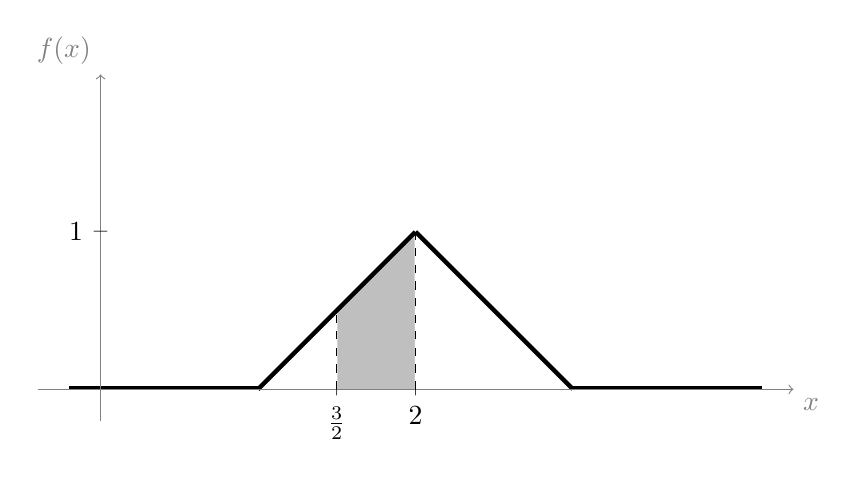
\begin{tikzpicture}[scale = 2]
		\draw[white, fill = gray!50, domain = 3/2:2, samples=200, smooth] (3/2,0)  -- plot (\x,{\x-1}) -- (2,0);
		\draw [ultra thick, fill=gray!50, domain = -0.2:1, samples=200, smooth] plot (\x,{0.01});
		\draw [ultra thick, fill=gray!50, domain = 1:2, samples=200, smooth] plot (\x,{\x-1});
		\draw [ultra thick, fill=gray!50, domain = 2:3, samples=200, smooth] plot (\x,{3-\x});
		\draw [ultra thick, fill=gray!50, domain = 3:4.2, samples=200, smooth] plot (\x,{0.01});
		\draw [gray, ->] (0,-0.2) -- (0,2) node [above left] {$f(x)$};
		\draw [gray, ->] (-0.4,0) -- (4.4,0) node [below right] {$x$};
		\draw [dashed] (3/2,0) -- (3/2,3/2-1);
		\draw [dashed] (2,0) -- (2,2-1);
		%\draw (1,0) node {\tiny{$|$}} node [below = 1mm] {$1$};
		\draw (3/2,0) node {\tiny{$|$}} node [below = 1mm] {$\frac{3}{2}$};
		\draw (2,0) node {\tiny{$|$}} node [below = 1mm] {$2$};
		\draw (0,1) node [rotate = -90] {\tiny{$|$}} node [left = 1mm] {$1$};
\end{tikzpicture}
\end{center}

\subsection{Cdf of a continuous distribution} \label{cdf(continuous)}
\noindent The cdf of a continuous distribution must satisfy the same following three conditions that must be satisfied by the cdf of a discrete distribution (see section \ref{cdf}):
\begin{itemize}
\item $F(x)$ is non-decreasing
\item As $x \rightarrow -\infty, F(x) \rightarrow 0$
\item As $x \rightarrow \infty, F(x) \rightarrow 1$
\end{itemize}

\noindent Recall that the cdf, $F(x)$, for a (discrete or continuous) random variable, $X$, is defined so that $F(x) = P(X \leq x)$. For a continuous random variable, this is given by the accumulation function introduced in section \ref{A(x)}. That is,

  	\bigskip
	
	\hfil\fbox{
	\begin{minipage}{0.45\columnwidth}{
	
	\vskip 0.05cm
	\begin{center}
	$\displaystyle{F(x) = P(X \leq x)  = \int_{-\infty}^x f(t) \; dt}$
	\end{center}
	}
	\end{minipage}}
	\bigskip
	\bigskip

\noindent In general, we use $F$ to represent an accumulation function; however, when dealing with continuous random variables we will always use $F$ to represent the cdf. In section \ref{indefinite integral}, under the heading, ``\textit{first part},'' we stated that, for any antiderivative, $\mathcal{F},$
\[
\int_a^b f(t) \; dt = \mathcal{F}(b) - \mathcal{F}(a).
\]
Note that $\mathcal{F}$ represents any antiderivative of $f$, while $F$ represents the cdf. In the same section, under the heading, ``\textit{second part},'' we discussed the fact that the accumulation function \textit{is} an antiderivative of $f$, hence the cdf, $F$, is an antiderivative of $f$. Since $F$ is an antiderivative of $f$, it follows that

  	\bigskip
	
	\hfil\fbox{
	\begin{minipage}{0.53\columnwidth}{
	
	%\vskip 0.05cm
	\begin{center}
	$\displaystyle{P(a < X < b) = \int_a^b f(t) \; dt = F(b) - F(a)}$
	\end{center}
	}
	\end{minipage}}
	\bigskip
	\bigskip

\noindent Which gives us a convenient way to calculate probabilities in terms of $F(x)$. \\

\noindent We have defined $P(a < X < b)$ to be the area under the graph of $f(x)$, along the interval $(a,b)$. The following sequence of graphs give a visual indication of the way that this area can be obtained from the cdf:
\begin{center}
\begin{minipage}{0.45\textwidth}
\begin{center}
	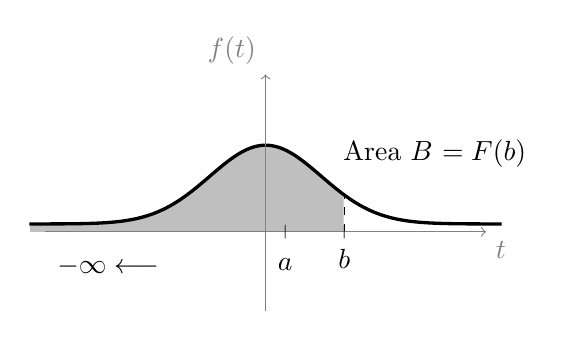
\begin{tikzpicture} [scale = 1]
	\draw[white, fill = gray!50, domain = -3:1, samples=200, smooth] (-3,0)  -- plot (\x,{exp(-(\x)^2) + 0.1}) -- (1,0);
	\draw [dashed] (1,0) -- (1,{exp(-(1)^2) + 0.1});
	\draw[very thick, domain = -3:3, samples=200, smooth] plot (\x,{exp(-(\x)^2) + 0.1});
	\draw [gray, ->] (0,-1) -- (0,2) node [above left] {$f(t)$};
	\draw [gray, ->] (-2.8,0) -- (2.8,0) node [below right] {$t$};
	\draw (-2,0) [below = 2mm] node {$-\infty \longleftarrow$};
	\draw (1,0) node {\tiny{$|$}} node [below = 1mm] {$b$};
	\draw (0.25,0) node {\tiny{$|$}} node [below = 2.2mm] {$a$};
	\draw (2.15,1) node {Area $B$ $= F(b)$};
	\end{tikzpicture}
\end{center}
\end{minipage}%
\begin{minipage}{0.45\textwidth}
\begin{center}
	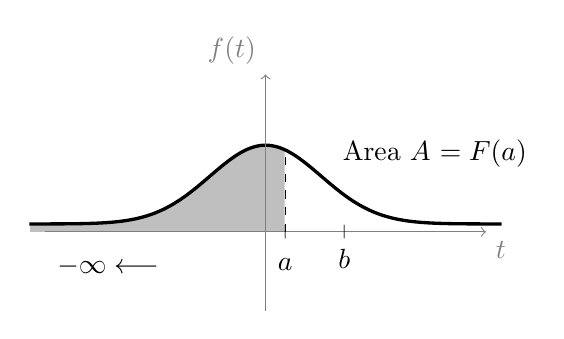
\begin{tikzpicture} [scale = 1]
	\draw[white, fill = gray!50, domain = -3:0.25, samples=200, smooth] (-3,0)  -- plot (\x,{exp(-(\x)^2) + 0.1}) -- (0.25,0);
	\draw[very thick, domain = -3:3, samples=200, smooth] plot (\x,{exp(-(\x)^2) + 0.1});
	\draw [gray, ->] (0,-1) -- (0,2) node [above left] {$f(t)$};
	\draw [gray, ->] (-2.8,0) -- (2.8,0) node [below right] {$t$};
	\draw [dashed] (0.25,0) -- (0.25,{exp(-(0.25)^2) + 0.1});
	\draw (-2,0) [below = 2mm] node {$-\infty \longleftarrow$};
	\draw (0.25,0) node {\tiny{$|$}} node [below = 2.2mm] {$a$};
	\draw (1,0) node {\tiny{$|$}} node [below = 1mm] {$b$};
	\draw (2.15,1) node {Area $A$ $= F(a)$};
	\end{tikzpicture}
\end{center}
\end{minipage}
\end{center}
Subtracting Area $A$ from Area $B$ gives
\begin{center}
	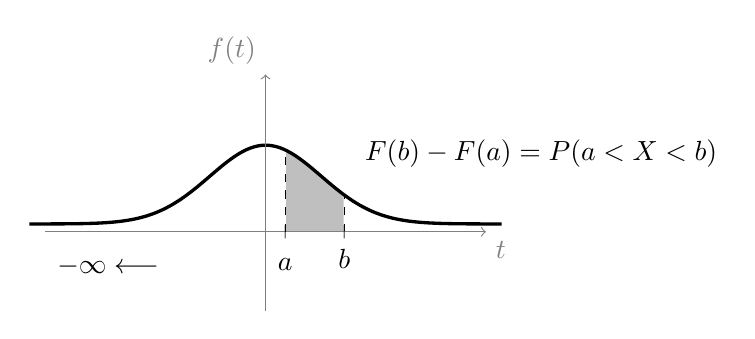
\begin{tikzpicture} [scale = 1]
	\draw[white, fill = gray!50, domain = 0.25:1, samples=200, smooth] (0.25,0)  -- plot (\x,{exp(-(\x)^2) + 0.1}) -- (1,0);
	\draw [dashed] (1,0) -- (1,{exp(-(1)^2) + 0.1});
	\draw[very thick, domain = -3:3, samples=200, smooth] plot (\x,{exp(-(\x)^2) + 0.1});
	\draw [gray, ->] (0,-1) -- (0,2) node [above left] {$f(t)$};
	\draw [gray, ->] (-2.8,0) -- (2.8,0) node [below right] {$t$};
	\draw (-2,0) [below = 2mm] node {$-\infty \longleftarrow$};
	\draw (1,0) node {\tiny{$|$}} node [below = 1mm] {$b$};
	\draw [dashed] (0.25,0) -- (0.25,{exp(-(0.25)^2) + 0.1});
	\draw (0.25,0) node {\tiny{$|$}} node [below = 2.2mm] {$a$};
	\draw (3.5,1) node {$F(b) - F(a) = P(a < X < b)$};
	\end{tikzpicture}
\end{center}

\noindent Finally, suppose that we are given the cdf, $F(x)$, of a continuous distribution, but we do not have the pdf, $f(x)$. Is there a way to obtain $f(x)$ from $F(x)$? \\

\noindent Since, as we just discussed, $F(x)$ is an antiderivative of $f(x)$, it follows that

  	\bigskip
	
	\hfil\fbox{
	\begin{minipage}{0.25\columnwidth}{
	
	\vskip 0.05cm
	\begin{center}
	$\displaystyle{\frac{d}{dx}\brac{F(x)} = f(x)}$
	\end{center}
	%\vskip 0.05cm
	}
	\end{minipage}}
	\bigskip
	\bigskip

\noindent So yes, we can obtain the pdf of a continuous distribution, once we know its cdf, by differentiating the cdf.

\section{Uniform distribution}
We now meet our first (and most basic) continuous distribution. Although it is simple, the uniform distribution is important in practice. Suppose we have a random variable, $X$, whose range is the interval $[c,d]$, with $c \neq d$. Then the random variable is uniformly distributed if and only if it has the following probability density function: \label{U(a,b)}

  	\bigskip
	
	\hfil\fbox{
	\begin{minipage}{0.52\columnwidth}{
	
	\vskip 0.05cm
	\begin{center}
	$\displaystyle{f(x) = \left\{ \begin{array}{ll}
\displaystyle{\frac{1}{d-c}}, & \;\; \text{if} \; x \in [c,d] \smallskip \\
0, & \;\; \text{otherwise}
\end{array} \right.}$
	\end{center}
	%\vskip 0.05cm
	}
	\end{minipage}}
	\bigskip
	\bigskip

\noindent Notice that $f(x) = \frac{1}{d-c}$ is constant for all $x \in [c,d]$. The values, $c$ and $d$, are the parameters of the distribution. We write \textbf{U$\boldsymbol{(c,d)}$} for short. We require $c \neq d$ since otherwise $d-c = 0$ (so we divide by zero). \\

\noindent Below is a graph of the uniform distribution:
\begin{center}
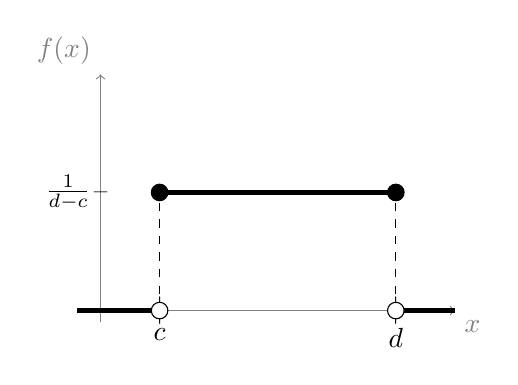
\begin{tikzpicture}[scale = 1.5]
\draw [gray, ->] (-0.1,0) -- (3,0) node [below right] {$x$};
\draw [gray, ->] (0,-0.1) -- (0,2) node [above left] {$f(x)$};
\draw (0.5,0) node {$|$} node [below = 1mm] {$c$};
\draw (2.5,0) node {$|$} node [below = 1mm] {$d$};
\draw [ultra thick] (0.5,1) -- (2.5,1);
\draw [fill = black] (0.5,1) circle (0.07cm);
\draw [fill = black] (2.5,1) circle (0.07cm);
\draw (0,1) node  [rotate = 90]  {\tiny{$|$}} node [left] {$\frac{1}{d-c}$};
\draw [ultra thick] (-0.2,0) -- (0.5,0);
\draw [ultra thick] (2.5,0) -- (3,0);
\draw [dashed] (0.5,0) -- (0.5,1);
\draw [dashed] (2.5,0) -- (2.5,1);
\draw [fill = white] (0.5,0) circle (0.07cm);
\draw [fill = white] (2.5,0) circle (0.07cm);
\end{tikzpicture}
\end{center}
If the distance from $c$ to $d$ is larger, then $d-c$ is also larger, so $\frac{1}{d-c}$ is smaller (so the graph is lower and wider). This makes sense since, as discussed in section \ref{pdf}, we must have
\[
\int_{-\infty}^\infty f(t) \; dt = 1,
\]
for any pdf. That is, the area under the graph must be the same (equal to 1) no matter what the distance is from $c$ to $d$.


\subsection{Example}
A parachutist lands at a random point on the line between two markers, $A$ and $B$, which are 50 meters apart. What is the probability that she lands closer to $A$ than to $B$? What is the probability that her distance to $A$ is more than four times her distance to $B$? \\

\noindent \textit{Solution:} \\
Let $X$ be the continuous random variable that measures her distance from marker $A$. Since we are told that she lands at a random point, we are going to assume that $X \sim$ U($c,d)$; for the parameters we will choose $c = 0$ (the position of $A$) and $d = 50$ (the position of $B$). The probability that she lands closer to $A$ than to $B$ is thus $P(X < 25) = F(25)$. We have
\begin{align*}
P(X < 25) = F(25) & = \int_{-\infty}^{25} f(t) \; dt \\
	& = \int_{-\infty}^0 f(t) \; dt + \int_0^{25} f(t) \; dt \tag{by formula (1) section \ref{integration}} \\
	& = 0 +  \int_0^{25} f(t) \; dt \tag{since $f(x) = 0$ when $x < 0$} \\
	& = \int_0^{25} \frac{1}{50} \; dt \tag{since $f(x) = \frac{1}{d-c} = \frac{1}{50-0}$ when $x \in [0,25]$} \\
	& = \squac{\frac{t}{50}}^{25}_0 \tag{FTC and an integral formula} \\
	& = \frac{25}{50} - \frac{0}{50} \\
	& = \frac{1}{2}.
\end{align*}
Now we wish to find the probability that her distance to $A$ is more than four times her distance to $B$. Let $b$ represent her distance from $A$. If she is 4 times closer to $B$, then she is at a distance $\frac{1}{4}b$ from $B$. Since the total distance ($A$ to $B$) is 50 meters, we know that \textit{distance to $A$} $+$ \textit{distance to $B$} = $b + \frac{1}{4}b = 50$. Solving for $b$ gives $b = 40$. Hence the probability that her distance to $A$ is \textit{more} than four times her distance to $B$ is given by
\begin{align*}
P(X > 40) & = 1 - P(X < 40) \tag{probability measure axiom 1} \\
	& = 1 - F(40) \\
	& =  1 - \int_{-\infty}^{40} f(t) \; dt \\
	& = 1 - \squac{\frac{t}{50}}^{40}_0 \tag{skipped steps that were the same as above} \\
	& = 1 - \brac{\frac{40}{50} - \frac{0}{50}} \\
	& = \frac{1}{5}.
\end{align*}
Notice that we used $P(X < 40) = F(40)$ and $P(X < 25) = F(25)$, when strictly speaking the definition of $F(x)$ is $F(x) = P(X \leq x)$. We cannot do this with discrete random variables, since the strictness of the inequality is important; however, for continuous random variables we have $P(X < x) = P(X \leq x)$, as discussed towards the end of section \ref{subsec15.1}.

\subsection{Cdf of uniform distribution} \label{sec15.2}
To find the cumulative distribution function for U($c,d$) we need to break the domain into separate parts: \\
\textbf{For $\boldsymbol{x < c:}$}
\[
F(x) = \int_{-\infty}^x 0 \; dt = 0 \tag{since $f(x) = 0$ for $x < c$} 
\]
\textbf{For $\boldsymbol{c \leq x \leq d:}$}
\begin{align*}
F(x) & = \int_{-\infty}^c 0 \; dt + \int_c^x \frac{1}{d-c} \; dt \tag{since $f(x) = \frac{1}{d-c}$ for $x \in [c,d]$} \\
	& = 0 + \squac{\frac{t}{d-c}}^x_c \tag{FTC and an integral formula} \\
	& = \frac{x}{d-c} - \frac{c}{d-c} \\
	& = \frac{x-c}{d-c}. \tag{$\bigstar$}
\end{align*}
\textbf{For $\boldsymbol{x > d:}$}
\begin{align*}
F(x) & = \int_{-\infty}^c 0 \; dt + \int_c^d \frac{1}{d-c} + \int_d^x 0 \; dt \tag{since $f(x) = 0$ for $c > d$} \\
	& = 0 + \frac{d-c}{d-c} + 0 \tag{substituting $x = d$ into ($\bigstar$)} \\
	& = 1.
\end{align*}
Hence
\[
F(x) = \left\{\begin{array}{ll}
0, & \;\; \text{if} \; x < c \smallskip \\
\frac{x-c}{d-c}, & \;\; \text{if} \; c \leq x \leq d \smallskip \\
1, & \;\; \text{if} \; x > d
\end{array} \right.
\]

\section{Inverse functions and percentiles} \label{cdf strictly increasing 1}
In section \ref{one to one} we mentioned that functions which are strictly increasing are always one-to-one (and hence they always have an inverse function). \\

\subsubsection{Median}
\noindent The cdf of a continuous random variable will always have an interval on which it increases, and one or more intervals on which it remains constant (flat); for example, the cdf of the uniform distribution (section \ref{sec15.2}) appears as follows
\begin{center}
\begin{tikzpicture}[scale = 1.5]
\draw[very thick, domain = 0.5:2.5, samples=200, smooth] plot (\x,{0.8*\x - 0.8*0.5});
\draw [gray, ->] (-0.1,0) -- (3.3,0) node [below right] {$x$};
\draw [gray, ->] (0,-0.1) -- (0,2.5) node [above left] {$f(x)$};
\draw [ultra thick] (2.5,0.8*2.5- 0.8*0.5) -- (3,0.8*2.5- 0.8*0.5);
\draw [ultra thick] (-0.2,0) -- (0.5,0);
\draw (0,0.8*2.5- 0.8*0.5) node [rotate = 90] {\tiny$|$} node [left] {$1$};
\draw [dotted] (2.5,0) -- (2.5,0.8*2.5 - 0.8*0.5);
\draw [dotted] (0,0.8*2.5 - 0.8*0.5) -- (2.5,0.8*2.5 - 0.8*0.5);
\draw (0.5,0) node {\tiny$|$} node [below = 1mm] {$c$};
\draw (2.5,0) node {\tiny$|$} node [below = 1mm] {$d$};
\end{tikzpicture}
\end{center}
As we can see, the cdf for U($c,d$) is strictly increasing on the interval $[c,d].$ Suppose that $F$ is the cdf of some arbitrary continuous random variable, and $I$ is the interval on which $F$ is increasing. To left of $I$ we get $F(x) = 0$, and to the right of $I$ we get $F(x) = 1$. \\

\noindent We can ask the question: For what value of $x \in I$ is $P(X \leq x) = 50\%$? This value, which we will label $x_m$, is called the \textbf{median}. \label{median} \\

\noindent We can find the median using the inverse of $F$, since
\[
F(x_m) = 0.5 \qquad \text{implies} \qquad x_m = F^{-1}(0.5)
\]

\subsubsection{Percentiles in general}
The $n^\text{th}$ \textbf{percentile} (also known as the $n^\text{th}$ \textbf{quantile}) is defined to be the value, $x_p$, below which $P(X \leq x_p) = n\%.$ By this definition, the median is the $50^\text{th}$ percentile. For $p = n/100$, we have
\[
P(X \leq x_p) = p \qquad \text{implies} \qquad x_p = F^{-1}(p)
\]

\subsection{Example}
What is the inverse function, $F^{-1}$, for the cdf of the uniform distribution, U($c,d$)? Hence find the median of U($c,d$). \\

\noindent \textit{Solution:} \\
The cdf only has an inverse for the interval, $I$, on which it is strictly increasing. For U($c,d$) we have $I = [c,d]$. Restricting $x$ to this interval we have
\[
F(x) = \frac{x-c}{d-c}. \tag{by the result in section \ref{sec15.2}}
\]
We use the method outlined in example \ref{ex9.inverse}, for finding inverse functions. \\
Let $F(x) = y$. Then $y \in [0,1]$ since this is the range of $F(x)$. Now,
\[
F^{-1}(y) = F^{-1}\brac{F(x)} = x \tag{by part (i) from the definition of inverse functions}
\]
So we have $F^{-1}(y) = x$. Now,
\begin{alignat*}{2}
&
& F(x)  
& = \frac{x-c}{d-c} \\
& \iff
& y
& = \frac{x-c}{d-c} \tag{since $y = F(x)$} \\
& \iff
& y(d-c)
& = x - c \\
& \iff
& y(d-c) + c
& = x \\
& \iff
& y(d-c) + c 
& = F^{-1}(y) \tag{since $x = F^{-1}(y)$}
\end{alignat*}
Now we can replace the dummy variable, $y$, with $x$, giving
\[
F^{-1}(x) = x(d-c) + c 
\]
Now we can find the median, $x_m$. We have
\[
F(x_m) = 0.5 = \frac{1}{2} \qquad \text{implies} \qquad F^{-1}\brac{\frac{1}{2}} = x_m.
\]
So
\[
x_m = F^{-1}\brac{\frac{1}{2}} = \frac{1}{2}(d-c) + c = \frac{1}{2}d - \frac{1}{2}c + c = \frac{c + d}{2}. 
\]
Below is a graph of the pdf of U($c,d$), displaying the median. The shaded part is $P(X \leq x_m)$; hence the shaded part has area $0.5$.
\begin{center}
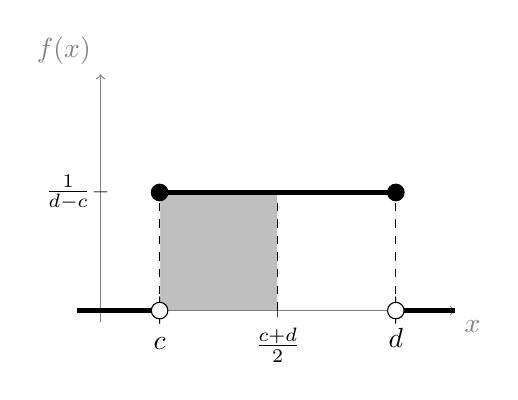
\begin{tikzpicture}[scale = 1.5]
\draw [white, fill = gray!50, domain = 0.5:1.5, samples=200,smooth] (0.5,0) -- plot (\x,1) -- (1.5,0);
\draw [gray, ->] (-0.1,0) -- (3,0) node [below right] {$x$};
\draw [gray, ->] (0,-0.1) -- (0,2) node [above left] {$f(x)$};
\draw (0.5,0) node {$|$} node [below = 2.2mm] {$c$};
\draw (2.5,0) node {$|$} node [below = 1mm] {$d$};
\draw [ultra thick] (0.5,1) -- (2.5,1);
\draw [fill = black] (0.5,1) circle (0.07cm);
\draw [fill = black] (2.5,1) circle (0.07cm);
\draw (0,1) node  [rotate = 90]  {\tiny{$|$}} node [left] {$\frac{1}{d-c}$};
\draw [ultra thick] (-0.2,0) -- (0.5,0);
\draw [ultra thick] (2.5,0) -- (3,0);
\draw [dashed] (0.5,0) -- (0.5,1);
\draw [dashed] (2.5,0) -- (2.5,1);
\draw [fill = white] (0.5,0) circle (0.07cm);
\draw [fill = white] (2.5,0) circle (0.07cm);
\draw (1.5,0) node {\tiny$|$} node [below = 1mm] {$\frac{c+d}{2}$};
\draw [dashed] (1.5,0) -- (1.5,1);
\end{tikzpicture}
\end{center}